\chapter{Implementazioni OpenMp: Prodotto Numerico}
\label{Chapter3}
%%%% 	ORGANIZZAZIONE
%{Accumulatore denso per i prodotti intermedi}	% breve remark da ch1, flags set per gestione inserimenti idx dups free, snippet di versione con partizionamento
%	{Trasformazione da un accumulatore denso in un vettore sparso}  % brevemenete approccio x passare (efficientemente) da formato denso a sparso
%		XXXX {Allocazione vettori sparsi intermedi} <-> integrare in:	Assegnamento dinamico di spazio per \nnz intermedi ai thread
%{Implementazioni con fase simbolica determinata con UpperBound}	giusto intro?
%   {Assegnamento dinamico di spazio per \nnz intermedi ai thread}  *alloc like atom x assegnare spazio pre allocato ai thread
%   {Assegnamento statico  di spazio per \nnz intermedi ai thread}	approccio con pre divisione (leggero overhead)
									%TODO CONFRONTO TRA I 2 -> teoricamente eguali (meno leggero overhead 2nd) a patto di dare ad ogni thread abbastanza spazio contiguo da fillare (false cache sharing)
%   {Consolidamento risultati intermedi nel risultato finale}	% mergeRows brevemente
%{Implementazioni con fase simbolica accurata} % remark sparisify diretto, implementato con funzione alla base del caso sparsify x versione UpperBound

	%dell'effettivo menziona il come è fatto con snippet semplificato
%{SpMM: Partizionamento monodimensionale}
%{SpMM: Partizionamento bidimensionale}

%{Sp3MM: Calcolo numerico diretto del triplo prodotto tra matrici}, remark approccio rowbyrowbyrow, ...?, snippet

%%%%

%----------------------------------------------------------------------------------------

Prendendo spunto dalle caratteristiche principali degli algoritmi descritti precedentemente in \ref{ChExistingTecqs}, 
in questa sezione vengono descritte implementazioni parallele derivate da gustavson \cite{gustavson} 
con formulazione row-by-row \ref{ChExistingTecqs:formulazioni} per il prodotto numerico tra matrici sparse con OpenMP, 
utilizzando diverse metodologie.
Estendendo l'approccio \rowbyrow, ho realizzato anche una versione per computare un triplo prodotto numerico direttamente.\\
%summing, organizzazione capitolo
In questo capitolo ho organizzato i contenuti per trattare prima dei componenti di supporto e configurazioni del prodotto numerico,
tra cui la differente gestione della memoria in base a quale tipo di prodotto simbolico si sta usando \ref{chSpMMSymb:UpperBound}.\\


\section{Accumulatore denso per le moltiplicazioni scalari intermedie} \label{chSpMMNum:scSparseVectMulPart}
%spiegazione dell'uso acc denso
Come precedentemente visto, una formulazione \rowbyrow di SpMM prevede di computare una riga di $C$ 
mediante la somma di moltiplicazioni scalari intermedie.\\
Analizzando gli ottimi risultati ottenuti da \cite{intelSpMMDenseAccumulator} precedentemente in 
\ref{ssec:intelSpMMDenseAccumulator}, ho deciso di sfruttare l'idea di utilizzare un accumulatore denso per 
sommare le moltiplicazioni scalari intermedie.\\
%double insert by intel paper...
Riguardo la determinazione degli indici di colonna degli elementi \nnz calcolati mediante l'accumulatore denso,
l'articolo menzionato \cite{intelSpMMDenseAccumulator} non specifica l'approccio usato nel dettaglio, 
ma solo che è possibile mantenere efficientemente gli indici inserendoli in un array quando l'elemento relativo nell'accumulatore denso era zero.\\
Tuttavia, quest'approccio è potenzialmente soggetto a reinserimenti di stessi indici in scenari in cui:
i valori \nnz della riga in uso di A comportano un particolare sequenziamento nelle somme delle moltiplicazioni scalari che portano
in una determinata entry dell'accumulatore denso a passare da zero a una serie di valori che 
passano nuovamente per zero (numerico). Date che la entry è tornata a zero, sommandoci un qualsiasi altro valore \nnz 
comporterà di dover reinserire il corrispondente indice.\\
%need my approch
Per quanto questo scenario è discretamente improbabile, %dato che lo zero numerico si ...
nel gestirlo si richiede di dover eliminare gli indici duplicati.\\
Al fine di evitare questa necessità, che potenzialmente richiede una ulteriore passata su tutti gli indici inseriti,
ho deciso di riutilizzare l'idea del set di flag usata per il prodotto simbolico in \ref{chSpMMSymb:structFlagSet}.\\
Ogni indice di colonna di elemento \nnz considerato durante la moltiplicazione scalare richiesta dalla formulazione \rowbyrow, 
verrà inserito in maniera del tutto analoga al caso del prodotto simbolico, incrementando un contatore se l'indice 
non era gia nella struttura ausiliaria di ricerca.\\
Le implementazioni delle bitmap per gestire set di flag saranno descritte in \ref{chSpMMAux:bitmapInsert}.\\
%TODO deconfusiona: reamrk o + ref a fatto che scSparseMul = moltiplicazione scalare è il 1° base step di \rowbyrow 
\begin{lstlisting}
typedef struct{
    double*  v;                     //nnz dense accumulator		(sparsellly filled)
    idx_t*   nnzIdx;                //v's nnz value's indexes		(contiguosily filled)
    idx_t    vLen;
    SPVECT_IDX_DENSE_MAP nnzIdxMap; //nnzIdx's indexed inserted flag set struct
} ACC_DENSE;
\end{lstlisting}
Nel frammento di codice precedente è riportata la struttura utilizzata come accumulatore denso per una riga della matrice risultante $C$.\\
In \vvv{v} saranno accumulati i valori \nnz relativi ad  ed i corrispondenti indici di colonna 
saranno copiati consecutivamente in \vvv{nnzIdx} e settati a \vvv{true} in \vvv{nnzIdxMap}.

\subsection{Trasformazione dell'accumulatore denso in un vettore sparso}	\label{chSpMMNum:sparsify}
L'accumulatore denso calcolato precedentemente deve essere trasformato in un formato sparso per poter essere 
inserito nella matrice target.\\
Per fare questa operazione di \emph{sparsificazione} efficientemente viene utilizzato il vettore degli indici di \vvv{nnzIdx},
come mezzo per accedere solamente alle locazioni dell'accumulatore denso \vvv{v} di interesse,
%Gli indici in \vvv{nnzIdx} si possono accedere direttamente con una \vvv{memcpy}.
%I relativi valori numerici in \vvv{v} devono essere acceduti in un ciclo scansionando gli indici in \vvv{nnzIdx},
come effettuato nel ciclo a riga 4 della seguente funzione.\\
\begin{lstlisting}
static inline void _sparsifyUB(ACC_DENSE* accV,SPACC* accSparse,idx_t startColAcc){
    idx_t nnz = accV->nnzIdxMap.len;
    sort_idx_t(accV->nnzIdx,nnz); //sort nnz idx for ordered write
    for (idx_t i=0,j;    i < nnz;   i++){
        j =  accV->nnzIdx[i];
        accSparse -> JA[i] = j + startColAcc;
        accSparse -> AS[i] = accV->v[j];
    }
    accSparse -> len = nnz;
}
\end{lstlisting}
Nel frammento di codice precedente è possibile notare anche come sia gestita 
la possibilità di convertire un accumulatore denso relativo ad una partizione di riga della matrice risultante, 
gestendo un shifting degli indici di colonna \nnz relativi mediante la variabile \vvv{startColAcc} a riga 6
(necessario per partizionamenti bidimensionali del lavoro come verrà approfondito in \ref{chSpMMNum:parti2D} ).\\
%sort need
Ordinando \vvv{nnzIdx} prima della sua copia nella struttura di destinazione, 
serve a produrre una matrice sparsa in output con indici degli elementi \nnz ordinati.
La necessità di tale operazione dipende dall'uso della matrice successivo al prodotto 
e nel caso CSR la distizione tra formato ordinato e non è riportata da \cite{adaptiveTilingSpMM}.\\
\begin{figure}[h!]
  \centering 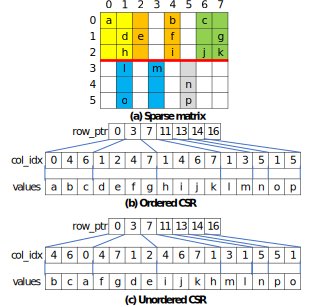
\includegraphics{csrOrderedAndUnordered.svg.png}
  \caption[Distinzione tra matrici CSR con indici di colonna in \vvv{JA} (non) ordinati]
  \decoRule \label{fig:layeredGraphInnerProduct}
\end{figure}
Il costo dell'ordinamento degli indici della matrice risultante è ammortizzato su ogni partizione di riga assegnata ad ogni thread.\\
Ho deciso di implementare l'ordinamento mediante l'implementazione di quicksort
presente nella \vvv{glibc} mediante la funzione \vvv{qsort}.\\


\section{Gestione della memoria in base al tipo di Prodotto Simbolico usato}
Come precedentemente detto in \ref{ChExistingTecqs:openMP_for_philosophy},
è sempre preferibile utilizzare pre allocazioni in luogo di allocazioni dinamiche 
in implementazioni parallele.\\
In base al tipo di fase simbolica effettuata, possono esserci diverse possibilità per 
pre-allocare la memoria per l'operazione di SpMM e successivamente assegnarne 
porzioni ai vari threads.\\
\subsection{Possibilità offerte al Prodotto Numerico, in base al livello di output del Prodotto Simbolico}
\label{chSpMMNum:funcsMultiImplePurpose}
I livelli di output del prodotto simbolico definiti in \ref{chSpMMSymb:outputDetailLevel}, 
permettono di effettuare il prodotto numerico con vari livello di 
partizionamento del lavoro e di uso della memoria:
\begin{itemize}
	\item un prodotto simbolico con output di livello 1 è sufficente a realizzare 
		  il prodotto numerico unicamente salvando i risultati intermedi in una struttura temporanea preallocata,
		  di cui porzioni vengono assegnate ai thread dinamicamente.
		  Dettagli di questo approccio saranno trattati a breve in \ref{chSpMMNum:mallocReplaceAssigns}
	\item un prodotto simbolico con output di livello 2 consente di effettuare il prodotto numerico
		  con partizionamento monodimensionale del lavoro, dove le righe della matrice risultante 
		  possono essere salvate in una struttura temporanea preallocata, di cui porzioni vengono assegnate 
		  staticamente ai thread o direttamente nella matrice risultante nel caso di prodotto simbolico accurato.
	\item un prodotto simbolico con output di livello 3 consente anche di effettuare il prodotto numerico
		  con un partizionamento bidimensionale del lavoro, dove similmente al punto precedente è possibile
		  scrivere le partizioni delle righe della matrice risultante direttamente 
		  in una struttura temporanea o nella matrice risultante se il prodotto simbolico è accurato.
\end{itemize}

\subsection{Uso di una fase simbolica determinata con UpperBound}
Nel caso di utilizzare una fase simbolica rapida basata su UpperBound in una implementazione parallela di SpMM
, come già menzionato in \ref{chSpMMSymb:UB_VS_SYMBACC},
è necessario utilizzare durante la fase numerica una struttura temporanea per salvare i risultati dei prodotti.\\
\label{chSpMMNum:UB_necessitaCopyBack}
Questa necessità è dovuta al fatto che ogni thread non ha informazione sulla esatta dimensione della porzione di
matrice da calcolare e quindi non può scrivere i suoi risultati direttamente nell'output dell'operazione di SpMM.\\
La struttura intermedia che ho utilizzato è composta da una coppia di aree di memoria
dimensionate con l'output della fase simbolica usata, destinate rispettivamente ai
valori dei \nnz e i relativi indici di colonna calcolati durante le moltiplicazioni scalari della fase numerica.\\
Nel seguito verranno indicate le aree per i \nnz e i relativi indici del risultato di SpMM rispettivamente come 
\emph{AS\_tmp JA\_tmp}.\\
\label{chSpMMNum:SPACC}	%keep track UB sparsified starts->lens for rowsMerge
Le partizioni di righe della matrice risultante calcolate verranno scritte da ogni thread
in aree contigue di questa struttura intermedia, salvandone gli indirizzi iniziali 
in questa struttura di supporto.\\
Per supportare l'operazione conclusiva di copia dei risultati intermedi nella matrice output all'operazione di SpMM 
(descritta in \ref{chSpMMNum:mergeRows}) viene utilizzata la seguente struttura:
\begin{lstlisting}
//Sparse vector accumulator
typedef struct{                                               
    double* AS;    //row part nnz values                                         
    idx_t*  JA;    //row part nnz indexes
    idx_t   len;   //rowLen
} SPACC;           
\end{lstlisting}
Nella struttura precedente, con una notazione CSR, si rappresenta un generico vettore sparso 
con \vvv{len} elementi \nnz in \vvv{AS} e relativi indici (di colonna nela caso CSR) in \vvv{JA}.
Il thread che avrà determinato una partizione di una riga della matrice target
scriverà i valori \nnz e i relativi indici in 2 blocchi di memoria della struttura temporanea,
annotandone i rispettivi indirizzi inziali nei puntatori \vvv{AS JA} e la lunghezza in \vvv{len}.\\
%dyn or static assign blocks
L'assegnazione delle aree di memoria della struttura intermedia per i risultati computati 
da ogni thread è gestita in modo dinamico o statico.
È possibile selezionare quest'ultimo approccio a tempo di compilazione in luogo dell'altro
definendo la macro \verb|SPARSIFY_PRE_PARTITIONING| con valore {TRUE}.\\

\subsubsection{Assegnamento dinamico di spazio per non zeri intermedi ai thread} \label{chSpMMNum:mallocReplaceAssigns}
Un approccio di assegnazione di porzioni di \emph{AS\_tmp JA\_tmp} simile ad effettuare allocazioni 
dinamiche, ma senza le criticità di performance citate in \ref{ChExistingTecqs:openMP_for_philosophy}
è il seguente.\\
\label{chSpMMNum:sparsifyMallocReplace}
Ogni thread che necessita di \emph{sparsificare} l'accumulatore denso determinato durante 
le moltiplicazioni scalari in un'area di memoria può incrementare {\bf{atomicamente}} un 
indice relativo alla fine dell'ultima area di memoria assegnata ad un qualsiasi altro thread,
catturandone il valore precedente.\\
\label{chSpMMNum:sparsifyMallocReplace_EASY_INTEGRATION_IN_EVERY_UB_PARTITIONING}
Questa soluzione di gestione dello spazio intermedio ha il vantaggio di richiedere quasi
nessuna informazione dal prodotto simbolico (è sufficiente un output di livello 1 secondo la numerazione descritta in \ref{chSpMMSymb:outputDetailLevel})
indipendentemente dal particolare tipo di partizionamento del lavoro che si sta utilizzando.\\
%code 
Segue la funzione per trasformare l'accumulatore denso in formato sparso con questo approccio.\\
\begin{lstlisting}
//row[Part] sparsified in a thread safe reserved area using atomics
static inline void sparsifyUBNoPartsBounds
  (SPMM_ACC* acc,ACC_DENSE* accV,SPACC* accSparse, ulong startColAcc){
    idx_t nnz = accV->nnzIdxMap.len;
    idx_t sparsifyStartV;
    sparsifyStartV = __atomic_fetch_add(&(acc->lastAssigned),nnz,__ATOMIC_ACQ_REL); 
    accSparse -> AS = acc->AS + sparsifyStartV;
    accSparse -> JA = acc->JA + sparsifyStartV;
    _sparsifyUB(accV,accSparse,startColAcc);
}
\end{lstlisting}
Nel frammento di codice precedente, è possibile vedere come a riga a 6 venga usata
la builtin di gcc \verb|__atomic_fetch_add| \cite{gcc10.1}
per riservare al thread corrente una porzione di memoria di \emph{AS\_tmp JA\_tmp}
a riga 7 e 8, per scrivere i risultati intermedi computati.\\
La primitiva \verb|__atomic_fetch_add| permette di incrementare una locazione 
di memoria, ritornandone il valore non incrementato.
Ulteriori dettagli su questo approccio e su alcune varianti saranno analizzati in \ref{chSpMMAux:atomicSegAssign}

\subsubsection{Assegnamento statico  di spazio per \nnz intermedi ai thread} \label{chSpMMNum:preSplitAS_JA_tmp}
Un'alternativa semplice all'approccio precedente (\ref{chSpMMNum:mallocReplaceAssigns}),
è quello di effettuare una suddivisione per ogni (partizione di) riga della matrice risultante
dello spazio allocato in \emph{AS\_tmp JA\_tmp}, così da consentire ad ogni thread 
di poter scrivere i propri risultati intermedi in una spazio non soggetto a race-conditions.\\
Per realizzare questo è necessario avere conoscenza di un UpperBound per ogni (partizione di)
riga della matrice risultante, e conseguentemente è necessario utilizzare un prodotto simbolico
con un livello di dettaglio dell'output di livello 2 (3), 
seguendo la nomenclatura introdotta nel capitolo precedente \ref{chSpMMSymb:outputDetailLevel}.\\

\subsubsection{Consolidamento risultati intermedi nel risultato finale} \label{chSpMMNum:mergeRows}
In conclusione all'operazione di SpMM con fase simbolica basata su UpperBound, 
è necessario raccogliere tutti i valori \nnz e i relativi indici,
calcolati nella struttura temporanea ( \emph{AS\_tmp JA\_tmp} ) nella matrice risultante di output.
Per fare questo è sufficiente copiare solo gli elementi \nnz scritti nella struttura temporanea
mediante le strutture ausiliare \vvv{SPACC}, descritte in \ref{chSpMMNum:SPACC}.\\
Segue la funzione per radunare tutti i risultati intermedi relativi a partizioni di righe della matrice 
risultante nell'output dell'operazione di SpMM.\\
\begin{lstlisting}
inline int mergeRowsPartitions(SPACC* rowsParts,spmat* mat,CONFIG* conf){
	//offsets for preparing copy 
    idx_t nzNum=0,j,rLen,idx,partsNum = mat->M * conf->gridCols;
    idx_t* rowsPartsOffsets; //partsNum offsets for each row's partitiong of mat
    for (idx_t r=0; r<mat->M; r++){	///count nnz entries offsets per row's part.
        for (j=0,rLen=0; j<conf->gridCols; j++){
            idx = IDX2D(r,j,conf->gridCols);
            rowsPartsOffsets[idx]=nzNum+rLen; //part start=prev accumulated end
            rLen += rowsParts[idx].len;
        }
        nzNum += rLen;
        mat->IRP[r+1] = nzNum;
		#ifdef ROWLENS
        mat->RL[r] = rLen;
		#endif
    }
    mat->NZ = nzNum;
	...
	//copy
    idx_t pLen; //omp for aux vars
    #pragma omp parallel for schedule(static) private(pLen)
    for (idx_t i=0;  i<partsNum; i++){
        pLen = rowsParts[i].len;
        memcpy(mat->AS + rowsPartsOffsets[i],rowsParts[i].AS,pLen*sizeof(*(mat->AS)));
        memcpy(mat->JA + rowsPartsOffsets[i],rowsParts[i].JA,pLen*sizeof(*(mat->JA)));
    }
    return EXIT_SUCCESS;
}
\end{lstlisting}
Come è possibile vedere nel frammento di codiceprecedente, l'operazione di copia dei risultati
intermedi nella matrice risultante è divisa in 2 fasi.\\
Tra riga 5 e 16, viene cumulata la dimensione di tutti i blocchi di \nnz computati
nel prodotto numerico in un vettore ausiliario \vvv{rowsPartsOffsets} e nella componente 
\vvv{IRP} della matrice risultante.\\
Successivamente la copia vera e propria avviene in parallelo 
a livello di singola partizione di riga risultante nel ciclo a riga 22 mediante delle \vvv{memcpy}.\\
Ad ogni iterazione si preleveranno i \nnz scritti nella struttura temporanea realativi
alla partizione $i~mod~ \verb|conf->gridCols|$-esima della $\left\lfloor \frac{i}{\text{conf} \rightarrow \text{gridCols}} \right\rfloor$
riga dalla struttura temporanea, copiandoli nella posizione appropriata della matrice risultante.\\



\subsection{Uso di una fase simbolica accurata}
Nel caso di utilizzare un Prodotto Simbolico accurato, è possibile \emph{sparsificare}
gli accumulatori densi ottenuti sommando le moltiplicazioni scalari \ref{chSpMMNum:scSparseVectMulPart}
direttamente nella matrice risultante.\\
Per fare questo è necessaria una piccola operazione di inizializzazione della matrice di output
andando a popolare il vettore \vvv{IRP}, con la cumulazione del \nnnz delle 
(partizioni di) righe determinato durante la fase simbolica.\\

%%%%%%%%%%%%%%%%%%%%%%%%  CORE NUMERICAL PRODUCT  %%%%%%%%%%%%%%%%%%%%%%%%%%%%%%
\section{Esecuzione del Prodotto Numerico}
In questa sezione verranno analizzate metodologie per effettuare l'operazione di SpMM in parallelo,
considerando vari approcci di suddivisione dei dati tra i thread.\\
%%%% diff _UB_ and _SymbNum_ version
Come già detto l'uso di una fase simbolica accurata o basata su UpperBound, discrimina la necessità 
o meno di dover utilizzare una struttura intermedia durante il prodotto numerico.
Oltre questo dettaglio non ci sono particolari differenze nelle due implementazioni della fase numerica
e per questo si analizzeranno nel seguito le implementazioni che sono supportate da un prodotto simbolico basato su UpperBound.\\
%rewind \rowbyrow + extra description + adattamento per partizionamento 2D
La formulazione \rowbyrow, come indicato in \ref{ChExistingTecqs:formulazioni}, 
calcola la riga $c_{i*}$ della matrice risultante sommando i vettori ottenuti dalle moltiplicazioni scalari tra:
gli elementi $a_{ik} \in a_{i*}$ della corrispondente riga della matrice $A$ e  
le righe di $b_{k*} \in B$ relativi agli indici di colonna $k$ degli elementi $a_{ik}$.
Questa operazione è esprimibile in maniera compatta come:\\
$c_{i*} = \sum\limits_{k \in I_i(A)}  a_{ik} \ast  b_{k*}$.\\
È possibile derivare il calcolo della partizione di colonne $c_z - c_w$ della riga $c_{i*}$
limitando le moltiplicazioni scalari $a_{ik} \ast  b_{k*}$ alle relative partizioni di colonne della matrice $B$. 
L'operazione appena descritta è esprimibile in maniera compatta seguendo la notazione introdotta \ref{notazione} come:\\
$c_{i~c_z-c_w} = \sum\limits_{k \in I_i(A)}  a_{ik} \ast  b_{k~c_z-c_w}$.\\

\subsection{Partizionamento monodimensionale}
Un semplice partizionamento delle matrici per parallelizzare SpMM, è quello di 
assegnare righe intere o blocchi di righe della matrice da calcolare $C$ ai thread.\\
%partitioning terminology
Nella terminologia introdotta precedentemente in \ref{ChExistingTecqs:workCube}, equivale ad
assegnare gruppi di Layers del cubo di lavoro ai vari threads.\\
Segue una parte del codice per effettuare l'operazione di SpMM con 
un partizionamento dei dati di blocchi di righe della matrice A e C:    \label{chSpMMNum:part1DGroup}
\begin{lstlisting}
    #pragma omp parallel for schedule(runtime) private(acc,startRow,block)
    for (b=0;   b < cfg->gridRows; b++){
        block		= UNIF_REMINDER_DISTRI(b,rowBlock,rowBlockRem);
        startRow	= UNIF_REMINDER_DISTRI_STARTIDX(b,rowBlock,rowBlockRem);
        acc			= accVects + omp_get_thread_num();
        for (ulong r=startRow;  r<startRow+block;  r++){
            for (ulong c=A->IRP[r]-OFF_F; c<A->IRP[r+1]-OFF_F; c++) 
                CAT(scSparseRowMul_,OFF_F)(A->AS[c], B, A->JA[c]-OFF_F, acc);
            //trasform accumulated dense vector to a CSR row, in a tmp storage struct
        	#if SPARSIFY_PRE_PARTITIONING == T
			_sparsifyUB(acc,outAccumul->accs+r,0);
			#else
        	sparsifyUBNoPartsBounds(outAccumul,acc,outAccumul->accs + r,0);
			#endif
            _resetAccVect(acc);   //rezero for the next A row
        }
    }
    ///merge sparse row computed before in output matrix
    if (mergeRows(outAccumul->accs,AB))    goto _err;
\end{lstlisting}
Nel frammento di codice precedente è possibile vedere come ogni thread determini 
il proprio blocco di righe su cui operare a riga mediante la macro \verb|UNIF_REMINDER_DISTRI_STARTIDX|,
che consente di determinare blocchi di dimensione il più uniforme possibile  
effettuando una suddivisione del resto della divisione intera tra il numero di righe e \vvv{cfg->gridRows},
ovvero il grado di partizionamento monodimensionale della matrice.
Maggiori dettagli e considerazioni a riguardo di quest'approccio di distribuzione saranno
descritti in \ref{chSpMMAux:UNIF_REMINDER_DISTRI}.\\
Nel ciclo a riga 6, il thread accumulerà le moltiplicazioni scalari nel suo accumulatore denso
determinato a riga 5, per poi \emph{sparsificarne} la riga risultante con
una politica di assegnamento statica o dinamica dello spazio temporaneo pre allocato,
rispettivamente a riga 11 o 13 (come affrontato rispettivamente in 
\ref{chSpMMNum:mallocReplaceAssigns} e \ref{chSpMMNum:preSplitAS_JA_tmp} ).\\
Dopo aver calcolato e \emph{sparsificato}, una riga della matrice risultante, è 
necessario resettare l'accumulatore denso relativo usato (riga 15).\\
Al termine del calcolo di tutte le righe, è necessario raccoglierle dallo spazio temporaneo usato
alla matrice risultante a riga 19 (come visto in \ref{chSpMMNum:mergeRows}).\\

\subsection{Partizionamento bidimensionale} \label{chSpMMNum:parti2D}
Un partizionamento 2D dell'operazione di SpMM è quello di assegnare ai threads 
blocchi bidimensionali della matrice C ottenuti dalla moltiplicazione di
blocchi di righe della matrice A e blocchi di colonne della matrice B.
Questa tecnica è stata rappresentata graficamente in \ref{fig:gustavsonRigheBlocksGraphicalIntel}.\\
%partitioning terminology
Nella terminologia introdotta precedentemente in \ref{ChExistingTecqs:workCube}, equivale ad
assegnare gruppi di fibers del cubo di lavoro ai vari threads.\\
%details now
In questo caso le moltiplicazioni scalari saranno limitate a partizioni di colonne di B,
conseguentemente è possibile utilizzare un accumulatore denso dimensionato sulla più grande
partizione di colonne di B da analizzare.\\
Ho deciso di seguire questo approccio per risparmiare allocazioni temporanee di memoria, 
al costo di dover gestire uno \emph{shifting} degl'indici introdotti nell'accumulatore denso
durante le operazioni di
somma di moltiplicazioni scalari e \emph{sparsificazione} degli accumulatori densi.\\
\label{chSpMMNum:csrColPartitioning}
Al fine di effettuare un partizionamento della matrice CSR B per blocchi di colonne 
ho realizzato due approcci, uno basato su una struttura ausiliaria di offset per accedere le partizioni della matrice originale
ed uno basato sul copiare la matrice in sotto matrici corrispondenti alle partizioni da accedere.
Dettagli sulle tecniche di partizionamento per colonne di una matrice CSR saranno analizzate
separatamente in \ref{chSpMMAux:csrColPartitioning}\\
Dal momento che il codice relativo all'uso di questi due approcci nel Prodotto Numerico è molto simile
segue una descrizione del caso più semplice basato sulla copia delle partizioni di B in sotto matrici.\\

\subsubsection{Partizionamento delle colonne di B in matrici separate}
Segue l'implementazione del Prodotto Numerico con partizionamento bidimensionale del lavoro,
sfruttando il partizionamento delle righe di A descritto in \ref{chSpMMNum:part1DGroup}
e il partizionamento per colonne di B che verrà descritto in \ref{chSpMMAux:csrColPartitioningAllocatd}
\begin{lstlisting}
    #pragma omp parallel for schedule(runtime) private(accV,accRowPart,...)
    for (tileID = 0; tileID < gridSize; tileID++){
        ///get iteration's indexing variables
        //tile index in the 2D grid of AB computation TODO OMP HOW TO PARALLELIZE 2 FOR
        t_i = tileID/cfg->gridCols;  //i-th row block
        t_j = tileID%cfg->gridCols;  //j-th col block
        //get tile row-cols group FAIR sizes
        rowBlock = UNIF_REMINDER_DISTRI(t_i,_rowBlock,_rowBlockRem); 
        startRow = UNIF_REMINDER_DISTRI_STARTIDX(t_i,_rowBlock,_rowBlockRem);
        startCol = UNIF_REMINDER_DISTRI_STARTIDX(t_j,_colBlock,_colBlockRem);
        
        colPart = colPartsB + t_j;
        accV = accVectors + tileID; 
         
        for (ulong r=startRow;  r<startRow+rowBlock;  r++){		///compute (A*B)[:t_i:][:t_j:]
            //iterate over nz col index j inside current row r
            //row-by-row restricted to colsubset of B to get AB[r][:colBlock:]
            for (ulong j=A->IRP[r]-OFF_F,c,bRowStart,bRowLen; j<A->IRP[r+1]-OFF_F; j++){
                //get start of B[A->JA[j]][:colBlock:]
                c = A->JA[j]-OFF_F; // column of nnz entry in A[r][:] <-> target B row
                bRowStart = colPart->IRP[c];
				#ifdef ROWLENS
                bRowLen   = colPart->RL[c];
				#else
                bRowLen   = colPart->IRP[c+1] - bRowStart;
				#endif
                CAT(scSparseVectMulPart_,OFF_F)(A->AS[j],colPart->AS+bRowStart,colPart->JA+bRowStart,
                    bRowLen,startCol,accV);
            }

            accRowPart = outAccumul->accs + IDX2D(r,t_j,cfg->gridCols);
			#if SPARSIFY_PRE_PARTITIONING == T
			_sparsifyUB(accV,accRowPart,startCol);
			#else
            sparsifyUBNoPartsBounds(outAccumul,accV,accRowPart,startCol);
			#endif
            _resetAccVect(accV);
        }
    }
    if (mergeRowsPartitions(outAccumul->accs,AB,cfg))  goto _err;
\end{lstlisting}
Ogni thread è delegato al calcolo di un blocco 2D della matrice C,
identificato dagl'indici \verb|t_i| \verb|t_j|, 
moltiplicando un blocco di righe della matrice A e un blocco di colonne della matrice B,
identificati dalle variabili in righe 8-12.\\
Come nel caso monodimensionale, i blocchi assegnati ai thread sono di dimensione il più possibile uniforme.\\
Nel ciclo a riga 15, il thread corrente computerà la \verb|t_j|-esima partizione della riga \verb|r| di C, 
in un accumulatore denso che verrà \emph{sparsificato} a riga 32-36,
tenendo traccia dell'indice inziale della partizione di B in \vvv{startCol} per gestire lo 
shifting degli indici necessario ad usare un accumulatore denso dimensionato alla 
partizione di riga più grande di B.\\
Infine, a riga 40, tutte le partizioni di righe calcolate verranno unificate dalla struttura 
temporanea \vvv{outAccumul} alla matrice di output \vvv{AB},
in maniera analoga al caso precedente monodimensionale.\\


\subsection{Sp3MM: Calcolo numerico diretto del triplo prodotto tra matrici}
Dato che il problema orinario da risolvere è il triplo prodotto tra matrici sparse per applicazioni come 
amg4psblas \cite{AMG4PSBLAS\_Git}, ho deciso di di supportare anche 
la fase numerica della moltiplicazione diretta tra 3 matrici sparse, con un estenzione della formulazione \rowbyrow.
%mediante un partizionamento 1D ed una fase simbolica basata su UpperBound.\\ %TODO SOLO EURISTICA FACILE TESTATA.
L'approccio che ho seguito è derivato dal lavoro di \cite{Sp3MM4AMG} 
ed è basato sul riuso diretto delle righe computate con la formulazione \rowbyrow,
per determinare le righe della matrice finale, senza l'ausilio di una matrice contente un'operazione di SpMM intermedia.\\ 
Nel seguito si seguirà la notazione introdota inizialmente riguardo il triplo prodotto tra matrici sparse (\ref{notazioneSp3MM}).\\
%Core summarizing steps for Sp3MM
Il primo passo per l'operazione di Sp3MM è calcolare la riga $\left( R \cdot AC_i \right)_{r*}$ 
sottoforma di accumulatore denso \vvv{accRAC}, sommando i risultati delle moltiplicazioni scalari relative alla formulazione \rowbyrow.\\
Successivamente, indicizzando \vvv{accRAC} esattamente come fatto nella \emph{sparsificazione} di SpMM (\ref{chSpMMNum:sparsify}),
è possibile ottenere la riga della matrice target ${AC_{i+1}}_{r*} = \left(R\cdot AC_i\cdot P\right)_{r*}$ 
reiterando l'operazione di SpMM tra la riga ottenuta sottoforma di accumulatore denso e la matrice $P$.\\
%code
Di seguito il blocco di codice principale per realizzare questa operazione.\\
\begin{lstlisting}
#pragma omp parallel for schedule(runtime) private(accRAC,accRACP,c)
for (ulong r=0;  r<R->M; r++){    //row-by-row-by-row formulation
    accRAC  = accVectorsR_AC  + omp_get_thread_num();
    accRACP = accVectorsRAC_P + omp_get_thread_num();
	//computing (tmp) R*AC r-th row
    for (idx_t j=R->IRP[r]-OFF_F; j<R->IRP[r+1]-OFF_F; j++)
        CAT(scSparseRowMul_,OFF_F)(R->AS[j], AC, R->JA[j]-OFF_F, accRAC);
    //forward the computed tmp row for the final matrix's row
    for (idx_t j=0; j<accRAC->nnzIdxMap.len; j++){
        c = accRAC->nnzIdx[j];    
        CAT(scSparseRowMul_,OFF_F)(accRAC->v[c],P,c,accRACP);
    }
\end{lstlisting}
Come è possibile vedere, la \vvv{r}-esima riga di $R\cdot AC_i$ ottenuta a linea 7 sotoforma di accumulatore denso,
viene immediatamente riusata per determinare la \vvv{r}-esima riga di $AC_{i+1}$ a linea 11,
indicizzandola come fatto dalle funzioni di \emph{sparsificazione} analizzate in precedenza,
nel ciclo a riga 9.\\
